\documentclass{article}
\usepackage{xcolor}
\usepackage{graphicx} % For including images
\usepackage{amsmath} % For mathematical symbols and equations
\usepackage{hyperref} % For hyperlinks
\usepackage{listings} % For including code snippets
\usepackage{amssymb}
\usepackage[a4paper, total={6in, 9in}]{geometry}

\title{Projet Linux}
\author{FOFANAH Mankoulani \and VANGEEBERGEN Augustin}

\date{\today}
\renewcommand \contentsname{Table des matières}
\begin{document}
	
	\maketitle
	
	\begin{figure}[h]
		\centering
		
\includegraphics[width=0.5\textwidth]{logo.png}
		\label{fig:logoheh}
	\end{figure}
	
	\begin{figure}[h]
		\centering
		\includegraphics[width=0.5\textwidth]{Gold\_AlmaLinux.jpg}	
		\label{fig:logoheh}
	\end{figure}
	
	\newpage


	\tableofcontents
	\newpage
	
	
	
	
	
	\section{Introduction}
	Dans le cadre de ce projet, nous avons pour objectif de configurer un serveur GNU/Linux. Nous avons le choix d'utiliser n'importe quelle distributon RedHat-like, par exemple Fedora, ou bien Alma, sur laquelle nous avons travaillé en cours. Ce point est important, pour pouvoir poser une question précise au professeur en cas de souci.
	
	Notre choix se porte donc sur Alma Linux, mais les scripts fonctionnant sous Alma fonctionnent théoriquement exactement de la même manière sous Fedora Linux et RHEL.
	
	L'OS fonctionnera dans une machine virtuelle, hébergée sur un HYPER-V de Windows. De cette manière, aussi bien un utilisateur Windows que linux pourra accéder aux différents services.
	
	Le but est de pouvoir gérer en ssh un serveur avec plein d'outilsutiles, et de pouvoir installer/désinstaller les services à souhait, diminuant ainsi la surface d'attaque.
	
	Nous devons donc gérer des services de partage de fichiers, serveur DNS, serveur Web ainsi que serveur temps.
	
	La dernière étape sera de sécuriser le serveur correctement, notamment en utilisant SELinux, et en définissant les polices d'utilisation correctes.
	
	\begin{center}Me when Linux on Windows :
	\end{center}
	\begin{figure}[h]
		\centering
		
\includegraphics[width=0.5\textwidth]{meme.png}
		\label{fig:meme}
	\end{figure}
	\newpage
	
	\subsection{Consignes professeur}
	
	Les consignes sont les suivantes : 
	
	\begin{itemize}
		\item Le serveur devra contenir un partage NFS qui permettra aux utilisateurs du réseaux local d’y stocker des fichiers.
		\item Un partage Samba permettra aux utilisateurs Windows d’accéder à ce même partage.
		\item Il faudra mettre en place un serveur Web, FTP, MySQL et DNS qui permettra un hébergement multiutilisateurs. Le FTP permettra à chaque utilisateur d’accéder à son dossier Web. Il faudra créer une zone dans le DNS pour nos sites. (Automatisation)
		\item Le DNS fera également office de DNS cache pour le réseau local.
		\item Vous mettrez en place un serveur de temps pour que les machines du réseau local puissent se synchroniser.
		\item Vous devrez pouvoir vous connecter en SSH au serveur et y effectuer des configurations. (sécurité !!!)
		\item Pour la sécurité :
		\begin{itemize}
			\item politique utilisateur
			\item quotas
			\item partitionnement et gestion disque (LVM et raid)
			\item Gestion backup(ou, comment,…)
			\item Maj, désactiver l’inutile.
			\item Antivirus, firewall, ….
		\end{itemize}
		\item Vous êtes l’administrateur de ce serveur agissez en conséquence :
		\begin{itemize}
			\item Documenter
			\item Automatiser (script)
			\item Soyez proactif
			\item Sécurisez
			\item Tester
		\end{itemize}
		\item Le travail sera réalisé par groupe de deux et évaluer par moi pendant la session de juin
		\item Il faudra une machine cliente pour effectuer les tests (Windows et Linux)
		\item Vous devrez me démontrer le fonctionnement des services en 15 minutes. Donc connaissez votre machine et vos configurations sur le bout des doigts. Vous aurez 10 minutes pour installer le tout.
		\item L’évaluation comptera pour 100\% des points. 
		
	\end{itemize}
	
	\newpage	
	
	\subsection{Roadmap}
	L'ensemble sera scripté pour coller à l'ensemble des cas d'utilisation. Voici donc la liste prévue de ces scripts (pour installer/désinstaller):
		\begin{itemize}
			\item Menu de sélection
			\item SSH config wizard
			\item File sharing install wizard
			\item Web server install wizard
			\item FTP server install wizard
			\item MySQL server 
			\item DNS server (+ cache + création de zone + serveur cache)
			\item Time server
			\item Sécurisation
			\item Backup
			\item Updates
			\item Partitionnement
		\end{itemize}
		Il est donc indispensable de se former au BASH, afin de savoir faire un bon TUI, ainsi que des commandes conditionnelles, selon les features qui sont/ne sont pas déjà installées.
		
		Le service SSH est indépendant des autres services. Le DNS, time server également.
		
		Cependant, les Serveurs Web, SQL et FTP doivent fonctionner en symbiose. C'est aussi le cas du NFS et SMB. Ce sera donc une personne qui s'occupera de ces services deux à deux.
	\subsection{Répartition des tâches}
	\begin{itemize}
		\item Augustin
		\begin{itemize}
			\item Rapport
			\item Menu TUI
			\item Serveur Web
			\item Serveur SQL
			\item Serveur FTP 
			\item Serveur SMB
			\item Serveur NFS
		\end{itemize}
		\item Mankou
		\begin{itemize}
			\item Connexion SSH
			\item Serveur NTP
			\item Serveur DNS
			\item Service de Backup
		\end{itemize}
	\end{itemize}
	
	
	
	
	
	
	
	\section{Code}
%	\subsection{Introduction au Bash}
%	Comme nous devons apprendre le Bash pour les scripts, voici une petite %synthèse simplifiée.
%	
%		Un code Bash doit toujours commencer par :
%	\begin{lstlisting}
%	#!/bin/bash
%	\end{lstlisting}		
	
%	Pour afficher du texte, on utiliser la commande "echo" :
%	\begin{lstlisting}
%	echo "Hello, world!"
%	\end{lstlisting}		

	
%	\begin{center}
%		Une variable va se déclarer comme ceci :
%	\end{center}
%	\begin{lstlisting}
%name="John"
%age=30
%	\end{lstlisting}

%	\begin{center}
%On accède à sa valeur comme ceci :
%\end{center}

%\begin{lstlisting}[language=bash, label={lst:bash-script}]
%# Access and print variables
%echo "Name: $name"
%echo "Age: $age"

%# You can also use the curly braces syntax
%echo "Name: ${name}"
%echo "Age: ${age}"
%\end{lstlisting}

%\begin{center}
%	Une condition va s'écrire comme ceci :
%\end{center}
	
%\begin{lstlisting}[language=bash, label={lst:bash-script}]
%if [ condition ]; then
%# Commandes executees si condition vraie
%else
%# Commandes executees si condition fausse
%fi
%
%\end{lstlisting}
	
	\subsection{Menu TUI}
	\subsubsection{Introduction}
	Nous avons besoin d'un menu qui reprenne la somme de tout notre travail. Le menu principal en TUI est un simple menu permettant de choisir le script concernant une manipulation spécifique d'un ou plusieurs services destiné(s) au serveur. Tout cela en une seule ligne de commande.

	\subsubsection{Explications}
	Le contenu du menu est connu à l'avance, nous pouvons donc imprimer chaque ligne de sélection de choix à l'écran.
	Une boucle maintient le menu à l'écran et regarde si une option est entrée. Si elle est valide, elle fait un chmod +x sur le script concerné,et le lance.
	\subsubsection{Utilisation du script}
L'utilisation du script est assez explicite, il suffit de lire la liste des options et sélectionner le caractère correspondant. Etant assez simple, le menu est également robuste et ne requiert pas de précautions d'usage particulières.


	\subsection{DNS}
	\subsubsection{Introduction}
	Un Domain Name Server (DNS) est un système de nommage hiérarchique et décentralisé pour ordinateurs, services et autres ressources connectées à internet ou à un réseau privé. Sa fonction est de traduire un nom de domaine facilement appréhendable en une adresse IP que les machines utilisent pour s'identifier sur un réseau.
	
	\begin{itemize}
	\item A Record : Mappe un nom de domaine à une adresse IPv4
	\item CNAME : Mappe un nom de domaine à un autre nom de domaine
	\item NS : Définit le serveur DNS autoritatif sur le domaine
	\item Pointer : Mappe une adresse IP à un nom de domaine
	\item MX :
	\item TXT :
	\item AAAA Record :
	\end{itemize}
	
	Un DNS cache quant à lui est un serveur DNS qui stocke les réponses DNS pour une certaine période de temps, à savoir la valeur Time To Live (TTL) des enregistrements DNS. Les requêtes DNS passent donc par ce serveur, et en cas d'absence de l'information dans sa base de données, celui-ci fera office de serveur DNS récursif.

	\subsubsection{Explications}
	
	\begin{enumerate}
	\item Configuration du DNS
	\item Configuration du DNC cache

	"Enable the zone-statistics yes; directive in the named.conf file to monitor server performance and activity1.
Generate a current snapshot of server statistics by issuing the rndc stats command1.
The data is dumped into the /var/cache/bind/named.stats file by default1.
To view the cached DNS records, dump the in-memory cache to a file for analysis using the command sudo rndc dumpdb -cache1.
The cache is typically located at /var/cache/bind/named_dump.db for Debian-based systems, and /var/named/data/ directory is used by RedHat-based systems1.	"
	
	\end{enumerate}	
	
	\subsubsection{Utilisation du script}

	\subsection{Partage SAMBA}
	\subsubsection{Introduction}
	\subsubsection{Explications}

	Premièrement le script va installer le package "samba", si ce n'est pas déjà fait.
	Il va ensuite donner le choix à l'utilisateur pour gérer son partage samba.
	 
	(afin de voir quels sont les utilisateurs existants, ainsi que les groupes et directories associés au(x) partage(s).)
	A noter que les utilisateurs samba ont par défaut besoin d'être associés à un utilisateur UNIX, même si les deux bases de données sont bien distinctes.
	Il va nous falloir un menu pour pouvoir éditer :
	\begin{itemize}
		\item Les utilisateurs :
		\begin{itemize}
			\item[\checkmark] Lister  
			\begin{itemize}
				\item[\checkmark] utilisateurs UNIX
				\item[\checkmark] utilisateurs samba
			\end{itemize}
			\item[\checkmark] Ajouter 
			\begin{itemize}
					\item[\checkmark] utilisateur UNIX
				\item[\checkmark] utilisateur samba 
			\end{itemize}
			\item Retirer
						\begin{itemize}
				\item utilisateur UNIX
				\item[\checkmark] utilisateur samba 
				\item [\checkmark] tous les utilisateurs samba (à part root)
			\end{itemize}
			\item Désactiver utilisateur samba
			\item Activer utilisateur samba
			\item Changer le mot de passe
		\end{itemize}	
	\end{itemize}
	\subsubsection{Utilisation du script}

	\subsection{Partage NFS}
	\subsubsection{Introduction}

	\subsubsection{Explications}
	Concu pour partager des fichiers entre OS de type Unix, 
	
	Montage d'un FS samba sous Unix :
	\texttt{mount -t smbfs -o} (voir annexes du cours de linux P78)
	\subsubsection{Utilisation du script}
	
	\newpage
	
	
	
	
	
	
	
	
	
	
	\subsection{Serveur Web}
	\subsubsection{Introduction}
	Le déploiement d'un serveur web sous alma (ou fedora) est décrit dans cet \href{https://docs.fedoraproject.org/en-US/fedora-server/services/httpd-basic-setup/}{\underline{article}}.
	
	\subsubsection{Explications}	
		
	Deux subdirectories sont utiles pour la configuration :
	\begin{itemize}
		\item \texttt{/etc/httpd/conf.d}
		
		Pour stocker la configuration des différents sites web
		\item \texttt{/etc/httpd/conf.modules.d}
		
		Pour les modules chargés dynamiquement
	\end{itemize}
	Historiquement, les données du site web sont par défaut stockées dans :
	\begin{itemize}
		\item \texttt{/var/www/}
	\end{itemize}
	Cependant, pour plusieurs sites, il existe deux méthodes.
	\begin{itemize}
		\item utiliser  le directory \texttt{/var/www/} et stocker les sites dans des subdirectories (facile pour SELinux, peu orthodoxe car modifie la configuration de base)
		\item utiliser le directory /srv et stocker les sites dans des subdirectories avec dans ceux-ci :
		\begin{itemize}
			 \item htdocs
			 \item webapps
			 \item mail
			 \item ...
		\end{itemize}
	\end{itemize}
	Nous utiliserons donc :
	\begin{itemize}
		\item \texttt{/srv/<DOMAINNAME>/} pour stocker les données relatives au domaine
		\item  \texttt{/srv/<DOMAINMANE>/htdocs/} pour les pages html statiques
	\end{itemize}
	\colorbox{yellow}{\textcolor{red}{!! A compléter pour le setup des LVM !!}}
	
	
	Il faut  ensuite installer le package httpd. Le manuel en ligne conseille d'installer les packages pour la gestion ssl et pour le monitoring de domaine.
	
	Il suffit ensuite de démarrer le service httpd et de l'enable avec systemctl.
	
	La page d'accueil par défaut ressemble à ceci sur AlmaLinux :
		\begin{figure}[h]
		\centering
		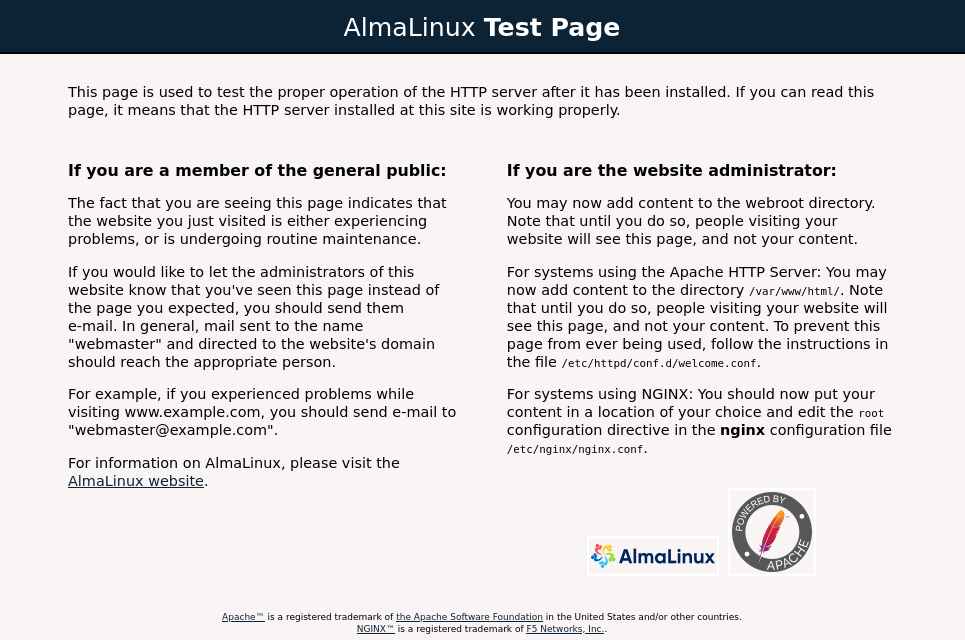
\includegraphics[width=0.8\textwidth]{webservdefault.png}
		 \caption{Page web par défaut sur Alma}
		\label{fig:your_label}
	\end{figure}
	
	Le menu de selection contient donc :
	\begin{itemize}
		\item Install web server
		\item Show httpd status
		\item Create web dir for user
		\item Remove web directory of user
		\item Display web directories
	\end{itemize}

	\subsubsection{Utilisation du script}	
	
	
	\newpage
	
	\subsection{Serveur SQL}
	\subsubsection{Introduction}
	\subsubsection{Explications}	
	\subsubsection{Utilisation du script}	

	\subsection{Serveur FTP}
	\subsubsection{Introduction}
	Le service FTP a été configuré à l'aide de cet \href{https://doc.fedora-fr.org/wiki/Vsftpd_:_Installation_et_configuration}{article de référence}.

	Chaque utilisateur spécifié doit être en mesure d'utiliser le service FTP pour accéder à :
	\begin{itemize}
		\item son dossier root
		\item son dossier web
	\end{itemize}

	\subsubsection{Explications}
	
	Le service choisi est vsftpd (Very Secure FTP Daemon). Il est le plus répandu au sein des distributions RedHat-like, peu gourmand, stable et sécurisé (d'où son nom).
	
	L'installation est similaire  celle du serveur web. Par conséquent, il faudra en premier installer le service, le démarrer et puis ensuite le configurer.
	
	Le fichier de configuration de vsftpd est : 
	\begin{center}
			\texttt{/etc/vsftpd/vsftpd.conf}
	\end{center}

	Dans ce fichier de configuration, on va choisir ces options :
	\begin{itemize}
	\item On écoute sur le port 21/tcp 
    \item On est en standalone 
    
Le mode standalone indique que le serveur est autonome, et que le service tourne en permanence. 
    \item On refuse les utilisateurs anonymes 
    \item On accepte les utilisateurs système et les utilisateurs virtuels 
    \item Les utilisateurs virtuels sont mappés sur l'utilisateur système "ftp" 
    \item Les utilisateurs n'ont aucun droit d'écriture par défaut 
    \item Ils sont chrootés dans:
    \begin{center}
		/var/ftp/
	\end{center}
    \item Le dossier pour les configurations d'utilisateurs virtuels :
    \begin{center}
 		/etc/vsftpd/vsftpd\_user\_conf/
	\end{center}
    \item La liste des utilisateurs refusés (pour lesquels on ne demandera même pas le mot de passe) sera contenue dans :
	\begin{center}
		/etc/vsftpd/user\_list
	\end{center}		
	\end{itemize}
	
	\subsubsection{Utilisation du script}
	
	Le menu présente diverses options :
	\begin{itemize}
		\item Install and enable ftp server
		\item Start ftp server 
		\item Stop ftp server
		\item Enable ftp server
		\item Disable ftp server 
		\item Show ftp server status
		\item Directory attribution for users :
		\begin{itemize}
			\item enable srv for all users
			\item enable home for all users
			\item  disable srv for all users
			\item disable home for all users
			\item enable srv for the specified user
			\item enable home for the specified user
		\end{itemize}
	\end{itemize}
	
	\newpage
	
	\subsection{Backup}
	Le menu Backup doit comporter deux options :
	\begin{itemize}
		\item Backup
		\item Restore
	\end{itemize}
	
	\newpage
	
	\subsection{Partitionnement}
	
	\newpage
	\section{Conclusion}


	\begin{figure}[h]
		\centering
		
\includegraphics[width=0.5\textwidth]{gosling.png}
		
		\label{fig:gosling}
	\end{figure}
	

	\begin{thebibliography}{9}
		\bibitem{reference1}
		Author, A. (Year). Title of the article. \textit{Journal Name}, Volume(Issue), Pages.
	\end{thebibliography}


\end{document}
